\documentclass{article}
\usepackage{graphicx} 
\usepackage[uft8]{ctex}
\usepackage{float} 
\usepackage{subfigure} 
\title{大数据分析云平台环境配置与测试}
\author{王艺羲 211250175}
\date{\today}

\begin{document}

\maketitle

\section{选择提供商}
选择阿里云作为提供商
\section{注册}
进行学生认证
\begin{figure}[ht]
    \centering
    
\includegraphics[width=\textwidth]{img/student.png}
    \caption{学生认证}
    \label{fig:enter-label}
\end{figure}

\section{创建实例}
创建云服务器实例
\begin{figure}[ht]
    \centering
    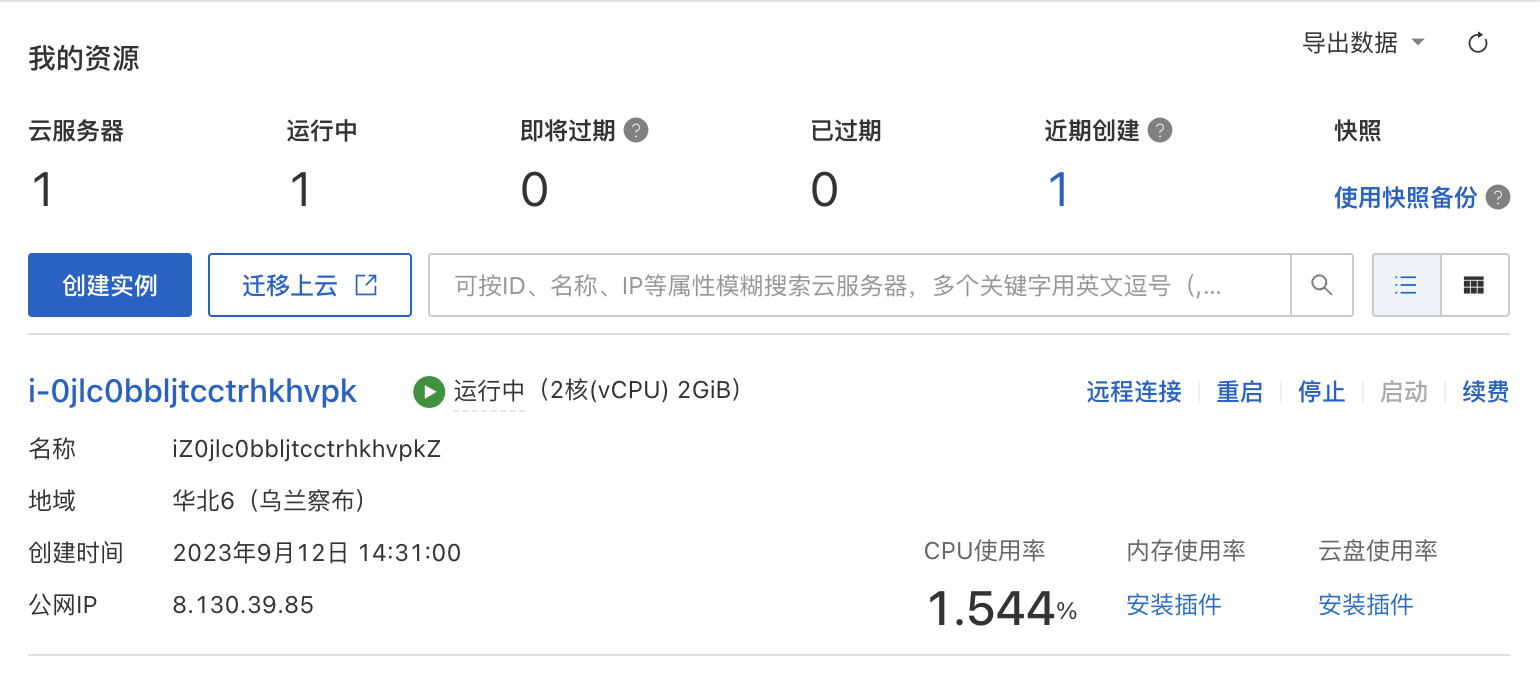
\includegraphics[width=\textwidth]{img/item.png}
    \caption{云服务器实例}
    \label{fig:enter-label}
\end{figure}

\section{基础测试}

\subsection{环境准备}
配置Java和Hadoop环境
\begin{figure}[ht]
    \centering
    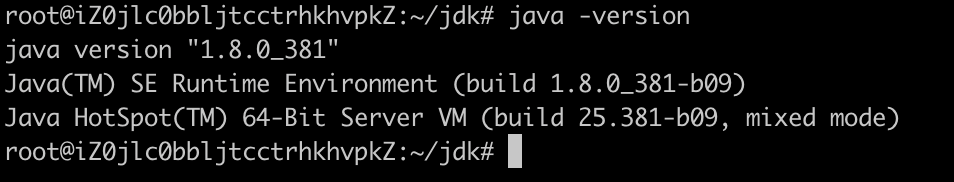
\includegraphics[width=\textwidth]{img/java.png}
    \caption{Java环境配置}
    \label{fig:enter-label}
\end{figure}

\begin{figure}[ht]
    \centering
    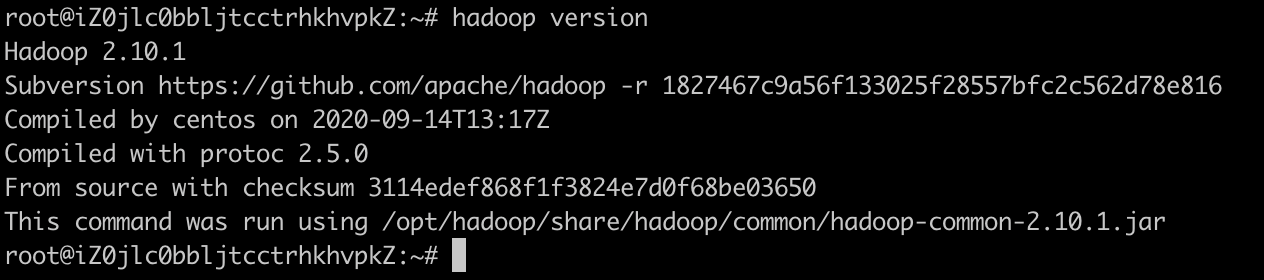
\includegraphics[width=\textwidth]{img/hadoop.png}
    \caption{Hadoop环境配置}
    \label{fig:enter-label}
\end{figure}

\subsection{代码编写}
使用Scala语言编写HellorWorld程序

\begin{figure}[ht]
    \centering
    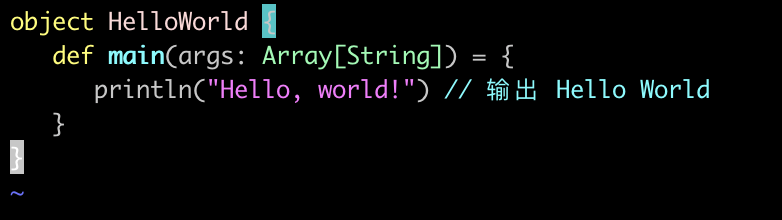
\includegraphics[width=\textwidth]{img/helloWorld.png}
    \caption{HelloWorld.scala}
    \label{fig:enter-label}
\end{figure}

\subsection{编译运行}
生成字节码并运行代码
\begin{figure}[ht]
    \centering
    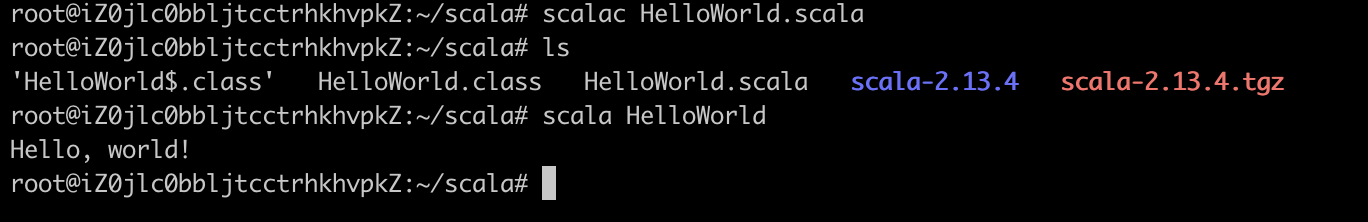
\includegraphics[width=\textwidth]{img/run.png}
    \caption{运行结果}
    \label{fig:enter-label}
\end{figure}

\subsection{结果验证}
输出为“Hello,world!”说明程序运行正常

\newpage
\section{清理}
终止实例或服务以避免额外收费。

\begin{figure}[ht]
    \centering
    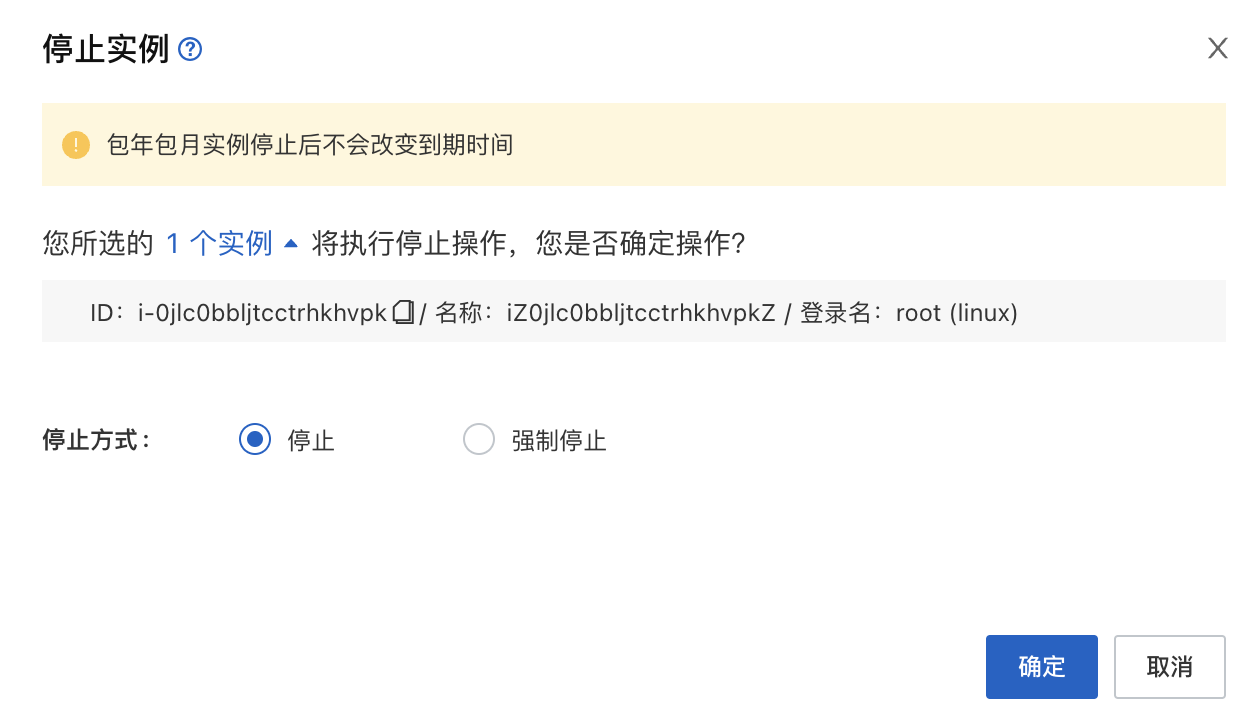
\includegraphics[width=\textwidth]{img/stop.png}
    \caption{运行结果}
    \label{fig:enter-label}
\end{figure}


\section{遇到的挑战及其解决方法}
挑战:如何向云服务器实例中导入下载好的JDK包
解决方法:下载FileZilla,打开在其中设置好服务器的公网ip地址、用户名、密码、端口等信息,远程连接服务器,向实例传输JDK压缩包

\end{document}
